%
% test file for building one chapter
%

\documentclass[12pt]{book}

\title{Think Java}
\author{Allen B. Downey and Chris Mayfield}

\newcommand{\thetitle}{Think Java}
\newcommand{\thesubtitle}{How to Think Like a Computer Scientist}
\newcommand{\theauthors}{Allen B. Downey and Chris Mayfield}
\newcommand{\theversion}{6.5.0 DRAFT}

%%%% Both LATEX and PLASTEX

\usepackage{graphicx}
\usepackage{setspace}
\usepackage{imakeidx}
\makeindex[options= -s headings.ist]

%BEGIN LATEX
\usepackage{comment}
\excludecomment{htmlonly}
\includecomment{latexonly}
%END LATEX

% automatically index glossary terms
\newcommand{\term}[1]{%
\item[#1:]\index{#1}}

\usepackage{amsmath}
\usepackage{amsthm}

% format end of chapter excercises
\newtheoremstyle{exercise}
  {12pt}        % space above
  {12pt}        % space below
  {}            % body font
  {}            % indent amount
  {\bfseries}   % head font
  {}            % punctuation
  {12pt}        % head space
  {}            % custom head
\theoremstyle{exercise}
\newtheorem{exercise}{Exercise}[chapter]

\newif\ifplastex
\plastexfalse

%%%% PLASTEX ONLY
\ifplastex

\usepackage{localdef}

\usepackage{url}

\newcount\anchorcnt
\newcommand*{\Anchor}[1]{%
  \@bsphack%
    \Hy@GlobalStepCount\anchorcnt%
    \edef\@currentHref{anchor.\the\anchorcnt}%
    \Hy@raisedlink{\hyper@anchorstart{\@currentHref}\hyper@anchorend}%
    \M@gettitle{}\label{#1}%
    \@esphack%
}

% code listing environments:
% we don't need these for plastex because they get replaced
% by preprocess.py
%\newenvironment{code}{\begin{verbatim}}{\end{verbatim}}
%\newenvironment{stdout}{\begin{verbatim}}{\end{verbatim}}

% inline syntax formatting
\newcommand{\java}{\verb}%}

%%%% LATEX ONLY
\else

\usepackage{geometry}
\geometry{
    width=5.5in,
    height=8.5in,
    hmarginratio=3:2,
    vmarginratio=1:1,
    includehead=true,
    headheight=15pt
}

% paragraph spacing
\setlength{\parindent}{0pt}                      % 17.62482pt
\setlength{\parskip}{12pt plus 4pt minus 4pt}    % 0.0pt plus 1.0pt
\linespread{1.05}
\def\arraystretch{1.5}

% list spacing
\setlength{\topsep}{5pt plus 2pt minus 3pt}      % 10.0pt plus 4.0pt minus 6.0pt
\setlength{\partopsep}{-6pt plus 2pt minus 2pt}  %  3.0pt plus 2.0pt minus 2.0pt
\setlength{\itemsep}{0pt}                        %  5.0pt plus 2.5pt minus 1.0pt

% these are copied from tex/latex/base/book.cls
% all I changed is afterskip
\makeatletter
\renewcommand{\section}{\@startsection{section}{1}{\z@}%
    {-3.5ex \@plus -1ex \@minus -.2ex}%
    {0.7ex \@plus.2ex}%
    {\normalfont\Large\bfseries}}
\renewcommand\subsection{\@startsection{subsection}{2}{\z@}%
    {-3.25ex\@plus -1ex \@minus -.2ex}%
    {0.3ex \@plus .2ex}%
    {\normalfont\large\bfseries}}
\renewcommand\subsubsection{\@startsection{subsubsection}{3}{\z@}%
    {-3.25ex\@plus -1ex \@minus -.2ex}%
    {0.3ex \@plus .2ex}%
    {\normalfont\normalsize\bfseries}}
\makeatother

% table of contents vertical spacing
\usepackage{tocloft}
\setlength\cftparskip{8pt plus 4pt minus 4pt}

% balanced index with TOC entry
\usepackage[totoc]{idxlayout}

% The following line adds a little extra space to the column
% in which the Section numbers appear in the table of contents
\makeatletter
\renewcommand{\l@section}{\@dottedtocline{1}{1.5em}{3.0em}}
\makeatother

% customize page headers
\usepackage{fancyhdr}
\pagestyle{fancyplain}
\renewcommand{\chaptermark}[1]{\markboth{Chapter \thechapter ~~ #1}{}}
\renewcommand{\sectionmark}[1]{\markright{\thesection ~~ #1}}
\lhead[\fancyplain{}{\bfseries\thepage}]%
      {\fancyplain{}{\bfseries\rightmark}}
\rhead[\fancyplain{}{\bfseries\leftmark}]%
      {\fancyplain{}{\bfseries\thepage}}
\cfoot{}
\usepackage[mmddyyyy]{datetime}
\rfoot{\textcolor{gray}{\tiny \thetitle, \theversion, \today}}

%% tweak spacing of figures and captions
%\usepackage{floatrow}
%\usepackage{caption}
%\captionsetup{
%    font=small,
%    labelformat=empty,
%    justification=centering,
%    skip=4pt
%}

% colors for code listings and output
\usepackage{xcolor}
\definecolor{bgcolor}{HTML}{FAFAFA}
\definecolor{comment}{HTML}{007C00}
\definecolor{keyword}{HTML}{0000FF}
\definecolor{strings}{HTML}{B20000}

% syntax highlighting in code listings
\usepackage{textcomp}
\usepackage{listings}
\lstset{
    language=java,
    basicstyle=\ttfamily,
    backgroundcolor=\color{bgcolor},
    commentstyle=\color{comment},
    keywordstyle=\color{keyword},
    stringstyle=\color{strings},
    columns=fullflexible,
    emph={label},  % keyword?
    keepspaces=true,
    showstringspaces=false,
    upquote=true,
    xleftmargin=15pt,  % \parindent
    framexleftmargin=3pt,
    aboveskip=\parskip,
    belowskip=\parskip
}

% code listing environments
\lstnewenvironment{code}
{\minipage{\linewidth}}
{\endminipage}
\lstnewenvironment{stdout}
{\lstset{commentstyle=,keywordstyle=,stringstyle=}\minipage{\linewidth}}
{\endminipage}

% interactive code listing
\lstnewenvironment{trinket}[2][400]
{\minipage{\linewidth}}
{\endminipage}

% inline syntax formatting
\newcommand{\java}[1]{\lstinline{#1}}%{

% prevent hyphens in names
\hyphenation{DrJava}
\hyphenation{GitHub}
\hyphenation{Javadoc}

% pdf hyperlinks, table of contents, and document properties
\usepackage{hyperref}
\hypersetup{%
  pdftitle={\thetitle: \thesubtitle},
  pdfauthor={\theauthors},
  pdfsubject={Version \theversion},
  pdfkeywords={},
  bookmarksopen=false,
  bookmarksnumbered=true,
  colorlinks=true,
  citecolor=black,
  filecolor=black,
  linkcolor=black,
  urlcolor=blue
}

% add dot after numbers in pdf bookmarks
\makeatletter
\renewcommand{\Hy@numberline}[1]{#1. }
\makeatother


\fi

%%%% END OF PREAMBLE
\begin{document}

\setcounter{chapter}{12}
\setcounter{page}{0}

\tableofcontents

\chapter{Objects of arrays}

\index{array!of cards}

In the previous chapter, we defined a class to represent cards and used an array of \java{Card} objects to represent a deck.
In this chapter, we take another step toward object-oriented programming by defining a class to represent a deck of cards.
We also present algorithms for shuffling and sorting decks.
Finally, we introduce \java{ArrayList} from the Java library and use it to keep track of which cards each player has from the deck.

%While reading the following sections, we recommend that you create a {\tt Deck.java} file and paste in all the examples.
%You will need {\tt Card.java} from the previous chapter for it to compile.

%So many of the examples are non-idiomatic; that is, they are not good Java.
%This transitional form should help you learn, but don't write code like this.

%The code for this chapter is in {\tt Card.java} and {\tt Deck.java}, which are in the directory {\tt ch13} in the repository for this book.
%Instructions for downloading this code are on page~\pageref{code}.


\section{The Deck class}
\label{deck}

The first goal of this chapter is to create a \java{Deck} class that encapsulates an array of \java{Card}s.
The initial class definition looks like this:

\begin{code}
public class Deck {
    private Card[] cards;

    public Deck(int n) {
        this.cards = new Card[n];
    }
    
    public Card[] getCards() {
        return this.cards;
    }
}
\end{code}

\index{constructor}
\index{memory diagram}
\index{diagram!memory}

The constructor initializes the instance variable with an array of \java{n} cards, but it doesn't create any \java{Card} objects.
Figure~\ref{fig.deckobject} shows what a \java{Deck} looks like with no cards.

\begin{figure}[!ht]
\begin{center}
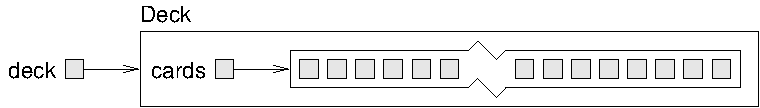
\includegraphics{figs/deckobject.pdf}
\caption{Memory diagram of an unpopulated \java{Deck} object.}
\label{fig.deckobject}
\end{center}
\end{figure}

We'll add another constructor that creates a standard 52-card array and populates it with \java{Card} objects:

\begin{code}
public Deck() {
    this.cards = new Card[52];
    int index = 0;
    for (int suit = 0; suit <= 3; suit++) {
        for (int rank = 1; rank <= 13; rank++) {
            this.cards[index] = new Card(rank, suit);
            index++;
        }
    }
}
\end{code}

This method is similar to the example in Section~\ref{cardarray}; we just turned it into a constructor.
We can now create a standard \java{Deck} like this:

\begin{code}
Deck deck = new Deck();
\end{code}

\index{printDeck}

Now that we have a \java{Deck} class, we have a logical place to put methods that pertain to decks.
Looking at the methods we have written so far, one obvious candidate is \java{printDeck} from Section~\ref{cardarray}.
Here's how it looks, rewritten as an instance method of \java{Deck}:

\begin{code}
public void print() {
    for (Card card : this.cards) {
        System.out.println(card);
    }
}
\end{code}

%\begin{code}
%public void print() {
%    for (int i = 0; i < this.cards.length; i++) {
%        System.out.println(this.cards[i]);
%    }
%}
%\end{code}

Notice that when you transform a static method into an instance method, the code is shorter.
We can simply type \java{deck.print()} to invoke this method.


\section{Shuffling decks}
\label{shuffle}

\index{shuffle}

For most card games, you need to be able to shuffle the deck; that is, put the cards in a random order.
In Section~\ref{random} we saw how to generate random numbers, but it is not obvious how to use them to shuffle a deck.

One possibility is to model the way humans shuffle, which is usually dividing the deck in two halves and then choosing alternately from each one.
Since humans usually don't shuffle perfectly, after about seven iterations the order of the deck is pretty well randomized.

But a computer program would have the annoying property of doing a perfect shuffle every time, which is not very random.
In fact, after eight perfect shuffles, you would find the deck back in the order you started in!
For more on this, see \url{https://en.wikipedia.org/wiki/Faro_shuffle}.

\index{pseudocode}

A better shuffling algorithm is to traverse the deck one card at a time, and at each iteration, choose two cards and swap them.
Here is an outline of how this algorithm works.
To sketch the method, we will use a combination of Java statements and English.
This technique is sometimes called {\bf pseudocode}.

\index{shuffle}

\begin{code}
public void shuffle() {
    for each index i {
        // choose a random number between i and length - 1
        // swap the ith card and the randomly-chosen card
    }
}
\end{code}

\index{helper method}
\index{method!helper}

The nice thing about pseudocode is that it often makes clear what other methods you are going to need.
In this case, we need a method that chooses a random integer between \java{low} and \java{high}, and a method that takes two indexes and swaps the cards at those positions.

\begin{code}
private static int randomInt(int low, int high) {
    // return a random number between low and high
}

private void swapCards(int i, int j) {
    // swap the ith and the jth cards in the array
}
\end{code}

\index{randomInt}
\index{swapCards}

Methods like \java{randomInt} and \java{swapCards} are called {\bf helper methods}, because they help you solve parts of the problem.
Helper methods are often \java{private}, since they are specific to the internal details of the class.

\index{top-down design}
\index{design process}

This process of writing pseudocode first and then writing helper methods to make it work is called {\bf top-down design} (see \url{https://en.wikipedia.org/wiki/Top-down_and_bottom-up_design}).
It is similar to ``incremental development'' and ``encapsulation and generalization'', the other design processes we have seen so far.

One of the exercises at the end of the chapter asks you to write the helper methods \java{randomInt} and \java{swapCards}, and use them to implement \java{shuffle}.


\section{Selection sort}
\label{sorting}

\index{selection sort}
\index{sort!selection}

Now that we have shuffled the deck, we need a way to put it back in order.
There is an algorithm for sorting that is ironically similar to the algorithm for shuffling.
It's called {\bf selection sort}, because it works by traversing the array repeatedly and selecting the lowest (or highest) remaining card each time.

During the first iteration, we find the lowest card and swap it with the card in the 0th position.
During the $i$th iteration, we find the lowest card to the right of $i$ and swap it with the $i$th card.
%Here is pseudocode for selection sort:

\begin{code}
public void selectionSort() {
    for each index i {
        // find the lowest card at or to the right of i
        // swap the ith card and the lowest card found
    }
}
\end{code}

Again, the pseudocode helps with the design of the helper methods.
For this algorithm we can use \java{swapCards} from before, so we only need a method to find the lowest card; we'll call it \java{indexLowest}.

\begin{code}
private int indexLowest(int low, int high) {
    // find the lowest card between low and high
}
\end{code}


One of the exercises at the end of the chapter asks you to write the helper method \java{indexLowest}; use it and \java{swapCards} to implement \java{selectionSort}.


\section{Merge sort}
\label{mergesort}

\index{efficiency}

Selection sort is a simple algorithm, but it is not very efficient.
To sort $n$ items, it has to traverse the array $n-1$ times.
Each traversal takes an amount of time proportional to $n$.
The total time, therefore, is proportional to $n^2$.

\index{merge sort}
\index{sort!merge}

In the next two sections, we'll develop a more efficient algorithm called {\bf merge sort}.
To sort $n$ items, merge sort takes time proportional to $n \log_2 n$.
That may not seem impressive, but as $n$ gets big, the difference between $n^2$ and $n \log_2 n$ can be enormous.

For example, $\log_2$ of one million is around 20.
So if you had to sort a million numbers, merge sort would require 20 million steps.
But selection sort would require one trillion!

The idea behind merge sort is this: if you have two subdecks, each of which has already been sorted, it is easy and fast to merge them into a single, sorted deck.
Try this out with a deck of cards:

\begin{enumerate}

\item Form two subdecks with about 10 cards each, and sort them so that when they are face up the lowest cards are on top.
Place both decks face up in front of you.

\item Compare the top card from each deck and choose the lower one.
Flip it over and add it to the merged deck.

\item Repeat step 2 until one of the decks is empty.
Then take the remaining cards and add them to the merged deck.

\end{enumerate}

The result should be a single sorted deck.
In the next few sections, we'll explain how to implement this algorithm in Java.


\section{Subdecks}

\index{subdeck}

The first step of merge sort is to split the deck into two subdecks, each with about half of the cards.
So we need to write a method, \java{subdeck}, that takes a deck and a range of indexes.
It returns a new deck that contains the specified subset of the cards.

\begin{code}
public Deck subdeck(int low, int high) {
    Deck sub = new Deck(high - low + 1);
    for (int i = 0; i < sub.cards.length; i++) {
        sub.cards[i] = this.cards[low + i];
    }
    return sub;
}
\end{code}

The first line creates an unpopulated subdeck (an array of \java{null} references).
Inside the \java{for} loop, the subdeck gets populated with references from the deck.

\index{off-by-one}

The length of the subdeck is \java{high - low + 1}, because both the low card and the high card are both included.
This sort of computation can be confusing, and forgetting the ``\java{+ 1}'' often leads to {\bf off-by-one} errors.
Drawing a picture is usually the best way to avoid them.

%For example, to select the middle three of five values in an array, we need \java{3 - 1 + 1} values.
%
%\begin{center}
%\begin{tabular}{ccccc}
%\hline
%\multicolumn{1}{|c|}{} & \multicolumn{1}{c|}{X} & \multicolumn{1}{c|}{X} & \multicolumn{1}{c|}{X} & \multicolumn{1}{c|}{} \\
%\hline
%0                      & 1                      & 2                      & 3                      & 4                     \\
%\end{tabular}
%\end{center}

\index{constructor}
\index{overload}

Figure~\ref{fig.subdeck} is a memory diagram of a subdeck with \java{low = 0} and \java{high = 4}.
The result is a hand with five cards that are {\em shared} with the original deck; that is, they are aliased.

\begin{figure}[!ht]
\begin{center}
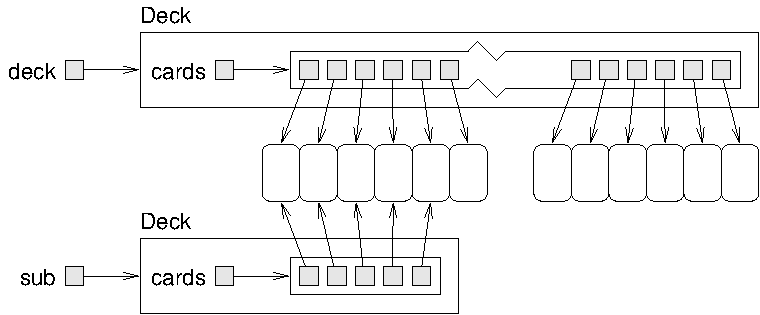
\includegraphics{figs/subdeck.pdf}
\caption{Memory diagram showing the effect of \java{subdeck}.}
\label{fig.subdeck}
\end{center}
\end{figure}

\index{aliasing}
\index{reference}

Aliasing might not be a good idea, because changes to shared cards would be reflected in multiple decks.
But since \java{Card} objects are immutable, this kind of aliasing is not a problem at all.
It also saves a lot of memory, because we never have to create duplicate \java{Card} objects.


\section{Merging decks}

The next helper method we need is \java{merge}, which takes two sorted subdecks and returns a new deck containing all cards from both decks, in order.
Here's what the algorithm looks like in pseudocode, assuming the subdecks are named \java{d1} and \java{d2}:

\begin{code}
private static Deck merge(Deck d1, Deck d2) {
    // create a new deck big enough for all the cards

    // use the index i to keep track of where we are at in
    // the first deck, and the index j for the second deck
    int i = 0;
    int j = 0;

    // the index k traverses the result deck
    for (int k = 0; k < d3.length; k++) {

        // if d1 is empty, use top card from d2
        // if d2 is empty, use top card from d1
        // otherwise, compare the top two cards

        // add lowest card to the new deck at k
        // increment i or j (depending on card)
    }
    // return the new deck
}
\end{code}

An exercise at the end of the chapter asks you to implement \java{merge}.
It's somewhat tricky, so be sure to test it with different subdecks.
Once your \java{merge} method is working corectly, you can use it to write a simplified version of merge sort:

\begin{code}
public Deck almostMergeSort() {
    // divide the deck into two subdecks
    // sort the subdecks using selectionSort
    // merge the subdecks, return the result
}
\end{code}


\section{Adding recursion}

Now that we have a way to \java{merge} two decks, the real fun begins!
The magical thing about merge sort is that it is inherently recursive.
Take another look at the pseudocode for \java{almostMergeSort} in the previous section.

At the point where you sort the subdecks, why should you invoke the slower method, \java{selectionSort}?
Why not invoke the spiffy new \java{mergeSort} method, the one you are in the process of writing?
Not only is that a good idea, it is {\em necessary} to achieve the $\log_2$ performance advantage.
\index{recursion}

To make \java{mergeSort} work recursively, you have to add a base case; otherwise it repeats forever.
A simple base case is a subdeck with 0 or 1 cards.
If \java{mergeSort} receives such a small subdeck, it can return it unmodified since it would already be sorted.

The recursive version of \java{mergeSort} looks something like this:

\begin{code}
public Deck mergeSort() {
    // if the deck has 0 or 1 cards, return it
    // divide the deck into two subdecks
    // sort the subdecks using mergeSort
    // merge the subdecks, return the result
}
\end{code}

\index{leap of faith}

As usual, there are two ways to think about recursive programs: you can think through the entire flow of execution, or you can make the ``leap of faith'' (see Section~\ref{leap_of_faith}).
This example might encourage you to make the leap of faith.

When you used \java{selectionSort} to sort the subdecks, you didn't feel compelled to follow the flow of execution.
You just assumed it works because you had already debugged it.
And all you did to make \java{mergeSort} recursive was replace one sorting algorithm with another.
There is no reason to read the program any differently.

Well, almost.
You might have to give some thought to getting the base case right and making sure that you reach it eventually.
But other than that, writing the recursive version should be no problem.


\section{Static context}

Figure~\ref{fig.deck} lists the methods we have discussed.
In UML diagrams, \java{private} methods begin with a minus sign (\java{-}), and \java{static} methods are underlined.

\begin{figure}[!ht]
\begin{center}
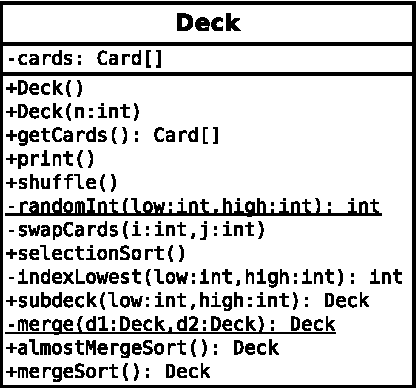
\includegraphics{figs/deck.pdf}
\caption{UML diagram for the \java{Deck} class.}
\label{fig.deck}
\end{center}
\end{figure}

The helper methods \java{randomInt} and \java{merge} are \java{static}, because they do not require \java{this.cards}.
All other methods are instance methods, because they require a specific instance of \java{this.cards}.
For example, you cannot invoke the \java{print} method this way:

\begin{code}
Deck.print();  // wrong!
\end{code}

\index{static context}
\index{this}

If you try to compile this code, you will get the error, ``non-static method print() cannot be referenced from a static context.''
By {\bf static context}, the compiler means you are trying to invoke a method without \java{this}.
To invoke an instance method, you need an instance:

\begin{code}
Deck deck = new Deck();
deck.print();  // correct
\end{code}

Notice that \java{Deck} with a capital \java{D} is a class, and \java{deck} with a lowercase \java{d} is a variable.
When you invoke \java{deck.print()}, the reference of \java{deck} becomes the reference \java{this}.
Static methods cannot refer to \java{this}, because they are not bound to a specific object.

\begin{code}
private static Deck merge(Deck d1, Deck d2) {
    return this.cards;  // wrong!
}
\end{code}

If you refer to \java{this} in a static method, you will get the compiler error, ``non-static variable this cannot be referenced from a static context.''
In static methods, there is no such thing as \java{this}.

\index{sort!Arrays}
\index{array!sorting}

Normally, we wouldn't implement three different sorting algorithms in the same class.
Our goal with \java{Deck} was to demonstrate different ways of solving the same problem.
In practice, we could just write a single \java{sort} method that uses \java{java.util.Arrays}.

\begin{code}
public void sort() {
    Arrays.sort(this.cards);
}
\end{code}

%%V6 Ex13.1
You can learn more about the sorting algorithms in this chapter, and others, at \href{http://www.sorting-algorithms.com/}{sorting-algorithms.com}.
This site includes explanations of the algorithms, animations that show how they work, and analysis of their efficiency.


\section{Piles of cards}

Now that we have a working \java{Deck} class, let's use it to implement a simple card game.
One of the simplest games that children often play is ``War'' (see \url{https://en.wikipedia.org/wiki/War_(card_game)}).

In this game, the deck is divided into two or more piles.
Players take turns revealing the top card of their pile.
If there is a tie, players set aside three more cards and reveal their next card.
Whoever has the highest ranking card takes all the cards that were played.
The game continues until one player has won the entire deck.

We could use the \java{Deck} class to represent the individual piles.
However, our implementation of \java{Deck} uses a \java{Card} array, and the length of an array can't change.
As the game progresses, we need to be able to add and remove cards from the piles.

\index{ArrayList}
\index{collection}

We can solve this problem by using an \java{ArrayList}, which is in the \java{java.util} package.
An \java{ArrayList} is a {\bf collection}, which is an object that contains other objects.
It provides methods to add and remove elements, and it grows and shrinks automatically.

%The Java library includes many other collections (see \url{https://docs.oracle.com/javase/8/docs/technotes/guides/collections/}).
%For our purposes, \java{ArrayList} is a good choice because it provides methods to add and remove elements, and it grows and shrinks automatically.

We will define a new class named \java{Pile} that represents a pile of cards.
It uses an \java{ArrayList} (instead of an array) to store the \java{Card} objects.

\begin{code}
public class Pile {
    private ArrayList<Card> cards;

    public Pile() {
        this.cards = new ArrayList<Card>();
    }
}
\end{code}

\index{angle brackets}

When you declare an \java{ArrayList}, you specify the type it contains in angle brackets (\java{<>}).
This declaration says that \java{cards} is not just an \java{ArrayList}, it's an \java{ArrayList} of \java{Card} objects.
The constructor initializes \java{this.cards} with an empty \java{ArrayList}.

%Java collections can only store objects, not primitives like \java{int}.
%But you can use wrapper classes, for example \java{ArrayList<Integer>}.

\java{ArrayList} provides a method, \java{add}, that adds an element to the collection.
We will write a \java{Pile} method that does the same thing:

\begin{code}
public void addCard(Card card) {
    this.cards.add(card);        // to the bottom of the pile
}
\end{code}

\index{this}

We also need to be able to remove cards from ``the top'' of the pile.
If we use \java{ArrayList.remove}, it will automatically shift the remaining cards left to fill the gap.

\begin{code}
public Card popCard() {
    return this.cards.remove(0);  // from the top of the pile
}
\end{code}

In order to know when to stop the game, we need to know how many cards are in each pile.

\begin{code}
public int size() {
    return this.cards.size();
}
\end{code}

\index{wrapper method}

Methods like \java{addCard}, \java{popCard}, and \java{size}, which invoke another method without doing much additional work, are called {\bf wrapper methods}.
The last method we need adds an entire subdeck at the beginning of the game.

\begin{code}
public void addDeck(Deck deck) {
    for (Card card : deck.getCards()) {
        this.cards.add(card);
    }
}
\end{code}

Now we can use \java{Deck} and \java{Pile} to implement the game.
In \java{War.java}, the \java{main} method begins like this:

\begin{code}
// create and shuffle the deck
Deck deck = new Deck();
deck.shuffle();

// divide the deck into piles
Pile p1 = new Pile();
p1.addDeck(deck.subdeck(0, 25));
Pile p2 = new Pile();
p2.addDeck(deck.subdeck(26, 51));
\end{code}

The game itself is a loop that repeats until one of the piles is empty.
At each iteration, we draw a card from each pile and compare their ranks.

\begin{code}
// while both piles are not empty
while (p1.size() > 0 && p2.size() > 0) {
    Card c1 = p1.popCard();
    Card c2 = p2.popCard();
    
    // compare the cards
    int diff = c1.getRank() - c2.getRank();
    if (diff > 0) {
        p1.addCard(c1);
        p1.addCard(c2);
    } else if (diff < 0) {
        p2.addCard(c1);
        p2.addCard(c2);
    } else {  // it's a tie...draw three more cards
\end{code}

One of the exercises at the end of this chapter asks you to implement the \java{else} block when there's a tie.
After the \java{while} loop ends, we display the winner based on which pile is not empty.

\begin{code}
if (p1.size() > 0) {
    System.out.println("Player 1 wins!");
} else {
    System.out.println("Player 2 wins!");
}
\end{code}

\java{ArrayList} provides many other methods that we didn't use for this example program.
You can read about them in the documentation, which you can find by doing a web search for ``Java ArrayList''.


\section{Vocabulary}

\begin{description}

\term{pseudocode}
A way of designing programs by writing rough drafts in a combination of English and Java.

\term{helper method}
Often a small method that does not do anything enormously useful by itself, but which helps another, more complex method.

\term{top-down design}
Breaking down a problem into sub-problems, and solving each sub-problem one at a time.

\term{selection sort}
A simple sorting algorithm that searches for the smallest or largest element $n$ times.

\term{merge sort}
A recursive sorting algorithm that divides an array into two parts, sorts each part (using merge sort), and merges the results.

\term{off-by-one}
A common programming mistake that results in iterating one too few (or too many) times.

%\term{insertion sort}
%Another sorting algorithm that inserts elements into place, one at a time.

\term{static context}
The parts of a class that run without reference to a specific instance of the class.

\term{collection}
An object that contains other objects, or more specifically, one of the objects in the Java library, like \java{ArrayList}, that contains objects.

\term{wrapper method}
A method that calls another method without doing much additional work.

\end{description}


\section{Exercises}

The code for this chapter is in the {\tt ch13} directory of {\tt ThinkJavaCode2}.
See page~\pageref{code} for instructions on how to download the repository.
Before you start the exercises, we recommend that you compile and run the examples.


\begin{exercise}  %%V6 Ex13.5

Write a \java{toString} method for the \java{Deck} class.
It should return a single string that represents the cards in the deck.
When it's printed, this string should display the same results as the \java{print} method in Section~\ref{deck}.

\index{StringBuilder}
\index{efficiency}

{\it Hint:} You can use the \java{+} operator to concatenate strings, but it is not very efficient.
Consider using \java{java.lang.StringBuilder} instead; you can review the documentation by doing a web search for ``Java StringBuilder''.

\end{exercise}


\begin{exercise}  %%V6 Ex13.2
\label{ex.shuffle}

The goal of this exercise is to implement the shuffling algorithm from this chapter.

\begin{enumerate}

\item In the repository for this book, you should find a file called {\tt Deck.java} that contains the code in this chapter.
Check that you can compile it in your environment.

\item Add a \java{Deck} method called \java{randomInt} that takes two integers, \java{low} and \java{high}, and returns a random integer between \java{low} and \java{high}, including both.
You can use the \java{nextInt} provided by \java{java.util.Random}, which we saw in Section~\ref{random}.

{\it Hint:} You can avoid creating a \java{Random} object every time \java{randomInt} is invoked by defining and using a class variable.


\item Write a method called \java{swapCards} that takes two indexes and swaps the cards at the given locations.

\item Write a method called \java{shuffle} that uses the algorithm in Section~\ref{shuffle}.

\end{enumerate}

\end{exercise}


\begin{exercise}  %%V6 Ex13.3

The goal of this exercise is to implement the sorting algorithms from this chapter.
Use the {\tt Deck.java} file from the previous exercise (or create a new one from scratch).

\begin{enumerate}

\item Write a method called \java{indexLowest} that uses the \java{compareCard} method to find the lowest card in a given range of the deck (from \java{lowIndex} to \java{highIndex}, including both).

\item Write a method called \java{selectionSort} that implements the selection sort algorithm in Section~\ref{sorting}.

\item Using the pseudocode in Section~\ref{mergesort}, write the method called \java{merge}.
The best way to test it is to build and shuffle a deck.
Then use \java{subdeck} to form two small subdecks, and use selection sort to sort them.
Then you can pass the two halves to \java{merge} to see if it works.
\index{testing}

\item Write the simple version of \java{mergeSort}, the one that divides the deck in half, uses \java{selectionSort} to sort the two halves, and uses \java{merge} to create a new, sorted deck.

\item Write a recursive version of \java{mergeSort}.
Remember that \java{selectionSort} is a modifier and \java{mergeSort} is a pure method, which means that they get invoked differently:

\begin{code}
deck.selectionSort();      // modifies an existing deck
deck = deck.mergeSort();   // replaces old deck with new
\end{code}

\end{enumerate}

\end{exercise}


\begin{exercise}  %%V6 Ex13.4

The goal of this exercise is to practice top-down design.
First read about ``insertion sort'' at \url{http://www.sorting-algorithms.com/insertion-sort}.
Then write a method named \java{insertionSort} that implements this algorithm.
Your method should use at least one helper method.

\end{exercise}


\begin{exercise}  %%V6.5 NEW

Open the file \java{War.java} in the repository.
The \java{main} method contains all the code from the last section of this chapter.
Check that you can compile and run this code before proceeding.

The program is incomplete; it does not handle the case when two cards have the same rank.
Finish implementing the \java{main} method beginning at the line that says: \java{// it's a tie...draw three more cards}.

When there's a tie, you need to draw three cards from each pile and store them in another collection.
Then draw one more card from each pile and compare them.
Whoever wins the tie will take all eight of these cards.

If one pile does not have at least four cards, the game ends immediately.
If a tie ends with a tie, flip a coin and give the cards to one of the players.

Notice that the program depends on \java{Deck.shuffle}.
If you haven't implemented the \java{shuffle} method (see Exercise~\ref{ex.shuffle}), every play will be a tie.
Player 1 will have the Ace through King of the first two suits, and Player 2 will have the the Ace through King of the remaining two suits, all in the same order.
As a result, the winner will be random.

\end{exercise}


\begin{exercise}  %%V6.5 NEW

Extend your program from the previous exercise to handle the case when a tie ends with a tie.
In other words, when the fourth cards have the same rank, add three more cards to the collection and try again.
You will need to wrap your code in a loop, for example: \java{while (diff == 0)}.

\end{exercise}


\end{document}
